\documentclass[UTF-8]{ctexbeamer}
\usetheme{Boadilla}

\usepackage{listing}
\usepackage[cache=false]{minted}

\title{Async Mechanism in Kernel Dev}
\subtitle{What, Why and How}

\author{王宇逸(Berrysoft) \& 刘晓义(喵喵)}
\date{2020-4}

\begin{document}
\begin{frame}
  \titlepage
\end{frame}

\begin{frame}
  \frametitle{First-class async in Rust}

  \begin{itemize}
    \item Async function, .await keyword
    \item Generators
    \item FSM: Finite yield point
  \end{itemize}

  \pause

  \vspace{1em}

  \textbf{Executors} poll futures to \textbf{make progress}

  Future providers use \textbf{Waker} to notify executors
\end{frame}

\begin{frame}[fragile]
  \frametitle{First-clas async in Rust: An example}

  \begin{minted}{rust}
    // async fn foo() -> u64
    async fn bar() -> u64 {
      set_timeout(1000).await;
      foo().await + 1
    }
  \end{minted}
  
  \pause
  \vspace{1em}
  Generates:
  \vspace{1em}

  \begin{minted}{rust}
    // enum Foo
    // enum Timeout
    enum Bar {
      Step1(Timeout),
      Step2(Foo),
      Finished(u64),
    }
  \end{minted}
\end{frame}

\begin{frame}[fragile]
  \begin{minted}{rust}
    enum Bar {
      Step1(Timeout),
      Step2(Foo),
      Finished(u64),
    }

    impl Future for Bar {
      type Output = u8;
      fn poll(self: Pin<&mut Self>, cx: &mut Context)
        -> Poll<u8> { match self { /* ... */ }}
    }
  \end{minted}

  \vspace{1em}

  {
    \centering
    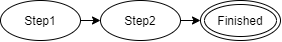
\includegraphics[width=0.5\textwidth]{assets/fsm.png}
  }
\end{frame}

\begin{frame}
  \frametitle{Future in Kernel}

  Schedulers are now \textbf{Executors}, and Threads are now \textbf{Top-level Futures}.

  \pause
  \vspace{1em}

  \begin{itemize}
    \item Saves kernel memory, prevents kernel stack overflow (State size/layout known at compile time)
    \item Unified wakeup interface
  \end{itemize}
\end{frame}

\begin{frame}
  \frametitle{Unified wakeup interface}

  How do we write \texttt{sleep}?

  \pause
  \vspace{1em}

  Traditionally:
  
  \begin{itemize}
    \item On sleep, thread push self into timer queue, and then yield.
    \item On wakeup, timer receives an interrupt, and pop corresponding thread.
  \end{itemize}

  \pause
  \vspace{1em}

  Now:

  \begin{itemize}
    \item impl Future<Item=()> for Timeout
    \item Timer::timeout() -> Timeout
  \end{itemize}
\end{frame}

\begin{frame}
  \frametitle{Executor}

  We need \textbf{Tasks, Wakers} and \textbf{Queues}.

  \pause
  \vspace{1em}

  \begin{itemize}
    \item \texttt{async-tasks}: Task abstraction
    \item \texttt{crossbeam}: Queues?
    \item \texttt{queueue}: Home-made queues
  \end{itemize}

\end{frame}

\begin{frame}
  \frametitle{Primitive Futures}

  \textbf{In zCore:} \texttt{sleep}, \texttt{yield\_now}

  \textbf{In rCore:} \texttt{timeout}, \texttt{wait\_int}, \texttt{channel} and sync primitives

  \pause
  \vspace{1em}

  Use combinators to form more complex structure
\end{frame}

\begin{frame}
  \frametitle{Hierarchy}

  \begin{figure}
    \centering

    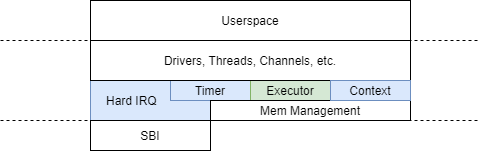
\includegraphics[width=0.8\textwidth]{assets/hierarchy.png}
  \end{figure}
\end{frame}

\begin{frame}
  \frametitle{Implementation}

  Basic executor implementation:

  \url{https://github.com/rcore-os-async/rcore-thread}

  \vspace{1em}

  Basic working kernel:

  \url{https://github.com/rcore-os-async/tutorial_port}

\end{frame}

\begin{frame}
  \frametitle{Q\&A}
\end{frame}
\end{document}
